\section{Clustering}
\label{sec:clustering}

All the \gls{ls} analysis methods presented so far rely on assumptions about a linear \gls{cs}.
For probing methods, concepts must be at least partially linearly separable for simple probes to detect them.
Latent direction methods posit that variations associated with a concept can be captured by moving along a linear axis of the \gls{ls}.
The \SuperpositionHypothesisName proposes that concepts are represented through linear directions that become entangled because of representational capacity constraints.
Although these assumptions have led to empirical successes, several observations suggest that the linearity hypothesis may not fully capture the \gls{cs}.

For instance, some concepts can only be recovered using non-linear probes.
Likewise, methods based on interpretable directions typically identify only a limited number of semantic factors.
Finally, in sparse autoencoder approaches, enforcing excessive sparsity degrades interpretability.
This suggests that the underlying representation may not be perfectly described by a sparse linear decomposition.
Taken together, these observations indicate that semantic concepts may not always exhibit a linear \gls{cs}.
This motivates the exploration of alternative approaches that rely on weaker assumptions regarding the geometry of \gls{ls}.

To the best of our knowledge, clustering-based analysis is the only family of \gls{ls} analysis methods that does not rely on any assumption of a linear \gls{cs} \cite{ren_deep_2022, wei_overview_2024}.
Rather than assuming that concepts correspond to directions, clustering methods only assume that conceptual similar inputs produce nearby \gls{lr}.
Conversely, inputs that differ significantly from a concept perspective are expected to be located farther apart in the \gls{ls}.
This is a considerably weaker assumption, in the sense that it is empirically verified in a wide range of settings.

Under this assumption, the discovery of concepts can be reformulated as the identification of groups of \gls{lr} that occupy the same region of the \gls{ls}.
This is shown schematically in Figure~\ref{fig:latent_clusters}, where the points represent \gls{lr} associated with concepts, and the ellipses indicate the approximate extent of each group and highlight their geometric separation.

\begin{figure}[t]
\centering

% ================================================================
%  latent_space_shared.tex
%  Couleurs, macros et styles partagés par toutes les figures
%  latent_space_*.tex
%  Usage : % ================================================================
%  latent_space_shared.tex
%  Couleurs, macros et styles partagés par toutes les figures
%  latent_space_*.tex
%  Usage : \input{figures/latent_space/latent_space_shared.tex}
% ================================================================

% ----------------------------------------------------------------
% Couleurs des clusters
% ----------------------------------------------------------------
\colorlet{colorA}{blue!70!cyan}
\colorlet{colorB}{orange}
\colorlet{colorC}{green!60!black}

% Couleurs de directions (latent_space_directions.tex)
\colorlet{colorDirBA}{violet}
\colorlet{colorDirBC}{red!70!black}

% ----------------------------------------------------------------
% Macros de dessin
% ----------------------------------------------------------------
\input{figures/latent_space/plot_points.tex}
\input{figures/latent_space/plot_ellipse.tex}
\input{figures/latent_space/plot_probe.tex}
\input{figures/latent_space/plot_direction.tex}

% ----------------------------------------------------------------
% Styles d'axe partagés
% ----------------------------------------------------------------
\pgfplotsset{
  % Axe standard (clustering, probing, directions)
  latent axis/.style={
    width=11cm,
    height=10cm,
    xmin=-7, xmax=8,
    ymin=-7, ymax=5.5,
    axis x line=bottom,
    axis y line=left,
    axis line style={
      -{Stealth[length=8pt, width=6pt]},
      thick
    },
    ticks=none,
    xlabel={},
    ylabel={},
    clip=true,
  },
  % Variante panneau carré (latent_space_sparse_autoencoders.tex)
  latent panel/.style={
    latent axis,
    width=9cm,
    height=9cm,
  },
  % Variante petit panneau (latent_space_embeddings.tex)
  % N.B. width/height sont passés explicitement par chaque fichier
  % via width=\lsePanelWd, height=\lsePanelHt dans l'axe.
  latent embed/.style={
    latent axis,
    every axis plot/.append style={forget plot},
  },
}

% ================================================================

% ----------------------------------------------------------------
% Couleurs des clusters
% ----------------------------------------------------------------
\colorlet{colorA}{blue!70!cyan}
\colorlet{colorB}{orange}
\colorlet{colorC}{green!60!black}

% Couleurs de directions (latent_space_directions.tex)
\colorlet{colorDirBA}{violet}
\colorlet{colorDirBC}{red!70!black}

% ----------------------------------------------------------------
% Macros de dessin
% ----------------------------------------------------------------
% ================================================================
%  \plotPoints — Reusable macro to render a point cloud from file
%
%  Usage:
%    \plotPoints[color=<c>, size=<s>, opacity=<o>]{<file.data>}
%
%  Arguments (all optional, defaults shown below):
%    color   : fill & stroke color of the markers  (default: black)
%    size    : marker radius                        (default: 2pt)
%    opacity : fill opacity [0..1]                  (default: 0.85)
%
%  Positional (mandatory):
%    #1 : path to a whitespace-separated x y data file
%         (lines starting with % are treated as comments)
%
%  Example:
%    \plotPoints[color=blue!70!cyan, size=3pt]{data/cluster_a.data}
% ================================================================
\pgfkeys{
  /plotPoints/.is family, /plotPoints,
  % --- defaults ---
  color/.initial   = black,
  size/.initial    = 2pt,
  opacity/.initial = 0.85,
}

\newcommand{\plotPoints}[2][]{%
  \pgfkeys{/plotPoints, #1}%                     % apply user overrides
  \pgfkeysgetvalue{/plotPoints/color}  {\ppColor}%
  \pgfkeysgetvalue{/plotPoints/size}   {\ppSize}%
  \pgfkeysgetvalue{/plotPoints/opacity}{\ppOpacity}%
  \addplot[
    only marks,
    mark        = *,
    mark size   = \ppSize,
    mark options= {fill=\ppColor, draw=\ppColor, fill opacity=\ppOpacity},
  ] file {#2};%
}
% ================================================================
%  \plotEllipse — Companion macro to draw a confidence ellipse
%
%  Usage:
%    \plotEllipse[color=<c>, width=<w>]
%                {<cx>}{<cy>}{<angle>}{<rx>}{<ry>}
%
%  Arguments (all optional):
%    color : stroke color  (default: black)
%    width : line width    (default: very thick)
%
%  Positional (mandatory):
%    {cx}    : ellipse center x  (axis coordinates)
%    {cy}    : ellipse center y  (axis coordinates)
%    {angle} : counter-clockwise rotation in degrees
%    {rx}    : horizontal semi-axis (cm)
%    {ry}    : vertical   semi-axis (cm)
%
%  Example:
%    \plotEllipse[color=orange]{-3}{1.5}{15}{2.3}{1.2}
% ================================================================
\pgfkeys{
  /plotEllipse/.is family, /plotEllipse,
  color/.initial = black,
  width/.initial = very thick,
}

\newcommand{\plotEllipse}[6][]{%
  \pgfkeys{/plotEllipse, #1}%
  \pgfkeysgetvalue{/plotEllipse/color}{\peColor}%
  \pgfkeysgetvalue{/plotEllipse/width}{\peWidth}%
  \draw[\peColor, \peWidth, rotate around={#4:(#2,#3)}]
    (#2,#3) ellipse (#5cm and #6cm);%
}
% ================================================================
%  plot_probe.tex — Linear probing decision boundary
%
%  \plotProbe[<options>]{<slope>}{<intercept>}
%
%  Draws  y = slope*x + intercept  clipped to the axis bounds.
%
%  Options (all optional):
%    color : line color   (default: black)
%    style : dash pattern (default: dashed)
%    width : line width   (default: thick)
%
%  WHY \edef ON THE WHOLE CALL: same deferred-rendering issue as
%  plot_points.tex — pgfplots evaluates ALL \addplot options at
%  \end{axis}, not at call time, so macro values must be baked in.
%
%  Example:
%    \plotProbe[color=colorA]{1}{3}
% ================================================================
\pgfkeys{
  /plotprobe/.is family, /plotprobe,
  color/.initial = black,
  style/.initial = dashed,
  width/.initial = thick,
}

\newcommand{\plotProbe}[3][]{%
  \pgfkeys{/plotprobe, #1}%
  \pgfkeysgetvalue{/plotprobe/color}{\prColor}%
  \pgfkeysgetvalue{/plotprobe/style}{\prStyle}%
  \pgfkeysgetvalue{/plotprobe/width}{\prWidth}%
  \edef\prDoPlot{%
    \noexpand\addplot[%
      domain=-7:8, samples=2,%
      \prStyle, \prWidth, color=\prColor, forget plot%
    ] {#2 * x + (#3)};%
  }%
  \prDoPlot
}

% ================================================================
%  plot_direction.tex — Interpretable direction vector
%
%  \plotDirection[<options>]{<x1>}{<y1>}{<x2>}{<y2>}
%
%  Draws a thick arrow from (x1,y1) to (x2,y2) in axis coordinates.
%  Must be called OUTSIDE the \addplot system, directly inside axis.
%
%  Options (all optional):
%    color   : arrow color   (default: black)
%    width   : line width    (default: very thick)
%    shorten : shorten tip   (default: 4pt)
%
%  Example:
%    \plotDirection[color=colorA]{-2.5}{-4}{-3}{1.5}
% ================================================================
\pgfkeys{
  /plotdirection/.is family, /plotdirection,
  color/.initial   = black,
  width/.initial   = very thick,
  shorten/.initial = 4pt,
}

\newcommand{\plotDirection}[6][]{%
  \pgfkeys{/plotdirection, #1}%
  \pgfkeysgetvalue{/plotdirection/color}  {\pdColor}%
  \pgfkeysgetvalue{/plotdirection/width}  {\pdWidth}%
  \pgfkeysgetvalue{/plotdirection/shorten}{\pdShorten}%
  \draw[\pdColor, \pdWidth, -Stealth,
        shorten >=\pdShorten, shorten <=\pdShorten]
    (axis cs:#2,#3) -- (axis cs:#4,#5);%
}


% ----------------------------------------------------------------
% Styles d'axe partagés
% ----------------------------------------------------------------
\pgfplotsset{
  % Axe standard (clustering, probing, directions)
  latent axis/.style={
    width=11cm,
    height=10cm,
    xmin=-7, xmax=8,
    ymin=-7, ymax=5.5,
    axis x line=bottom,
    axis y line=left,
    axis line style={
      -{Stealth[length=8pt, width=6pt]},
      thick
    },
    ticks=none,
    xlabel={},
    ylabel={},
    clip=true,
  },
  % Variante panneau carré (latent_space_sparse_autoencoders.tex)
  latent panel/.style={
    latent axis,
    width=9cm,
    height=9cm,
  },
  % Variante petit panneau (latent_space_embeddings.tex)
  % N.B. width/height sont passés explicitement par chaque fichier
  % via width=\lsePanelWd, height=\lsePanelHt dans l'axe.
  latent embed/.style={
    latent axis,
    every axis plot/.append style={forget plot},
  },
}


\resizebox{0.65\textwidth}{!}{
\begin{tikzpicture}
\begin{axis}[latent axis]

  % Cluster boundaries
  \plotEllipse[color=colorA, width=very thick, fill=colorA, fillopacity=0.08]
    {-3}{1.5}{15}{2.3}{1.2}
  \plotEllipse[color=colorB, width=very thick, fill=colorB, fillopacity=0.08]
    {-2.5}{-4}{10}{2.2}{1.1}
  \plotEllipse[color=colorC, width=very thick, fill=colorC, fillopacity=0.08]
    {4.2}{-0.5}{-20}{1.4}{2.6}

  % Point clouds
  \plotPoints[color=colorA, mark=*]{figures/latent_space/cluster_a.data}
  \plotPoints[color=colorB, mark=square*]{figures/latent_space/cluster_b.data}
  \plotPoints[color=colorC, size=2pt, mark=triangle*]{figures/latent_space/cluster_c.data}

\end{axis}
\end{tikzpicture}
}

\caption{
  Visualization of the latent space structure.
  The points represent embeddings associated with concepts A, B, and C.
  The ellipses indicate the approximate extent of each group in the latent space and highlight their geometric separation.
}
\label{fig:latent_clusters}
\end{figure}


This idea forms the basis of the research field known as deep clustering.
In these approaches, a collection of inputs is projected into a \gls{ls} using a \gls{nn}.
The resulting \gls{lr} form a point cloud on which standard clustering algorithms can be applied.
The obtained clusters are then interpreted as representing distinct concepts.

Deep clustering has been particularly successful in unsupervised image classification.
For this type of task, a specific \gls{nn} architecture called an autoencoder is commonly used.
An autoencoder is composed of an encoder $f_{\text{enc}}$ and a decoder $f_{\text{dec}}$.
The encoder maps an input $x \in \mathcal{X}$ to a low-dimensional \gls{lr} $\mathbf{z} \in \mathbb{R}^d$, the \gls{lr} produced by the encoder.
The decoder then maps this \gls{lr} back to the input space to produce a reconstruction $\hat{x}$.
The model is trained by \gls{sgd} to minimize the reconstruction error between the original input and its reconstruction using a \gls{mse} loss.
This objective encourages the \gls{ls} to preserve the most informative features of the input while enforcing a compact representation.
This can be expressed mathematically as follows:
\[
x
\xrightarrow{\;f_{\mathrm{enc}}\;}
\mathbf{z}
\xrightarrow{\;f_{\mathrm{dec}}\;}
\hat{x},
\qquad
d \ll \dim(\mathcal{X}),
\qquad
\mathcal{L}_{\mathrm{rec}}
=
\frac{1}{N}\sum_{i=1}^{N}
\left\|x^{(i)}-\hat{x}^{(i)}\right\|_2^2.
\]

Once the autoencoder has been trained sufficiently well, the reconstruction loss $\mathcal{L}_{\mathrm{rec}}$ should be low enough for the learned representation to be useful.
A clustering algorithm can then be applied to the compressed representations of the images.
Let $\mathcal{D}$ denote a dataset of inputs, through the encoder $f_{\text{enc}}$, this dataset is mapped to a point cloud in the \gls{ls}:
$$
\mathcal{Z} = \{\mathbf{z}^{(i)} \in \mathbb{R}^d \mid \mathbf{z}^{(i)} = f_{\text{enc}}(x^{(i)}), \; x^{(i)} \in \mathcal{D} \}.
$$

A classical clustering algorithm is applied to the set $\mathcal{Z}$ of \gls{lr} to identify groups of similar \gls{lr}.
Each resulting cluster can therefore be interpreted as a group of images that the model considers similar.

An example of this methodology can be observed in Figure~\ref{fig:deep_clustering_illustration}, where the approach is applied to the STL-10 dataset \cite{coates2011analysis} using $k$-means clustering \cite{macqueen1967multivariate} with a number of clusters arbitrarily fixed to $K = 10$ \cite{xie_unsupervised_2016}.
For each cluster, the corresponding line shows the $10$ samples closest to the associated centroid in the \gls{ls}.

\begin{figure}[t]
    \centering
    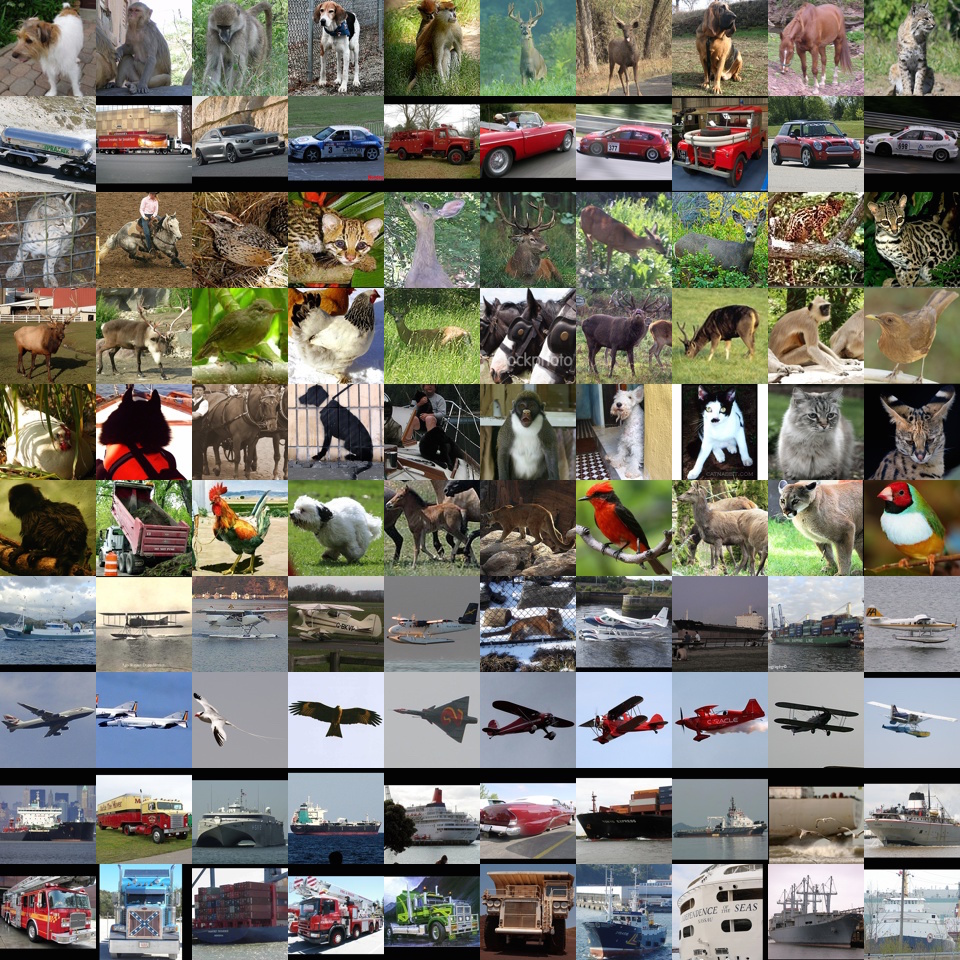
\includegraphics[width=0.85\textwidth]
        {figures/latent_space/deep_clustering_illustration.jpg}
    \caption{
        Clusters discovered by a deep clustering model applied to natural images \cite{xie_unsupervised_2016}.
    }
    \label{fig:deep_clustering_illustration}
\end{figure}

We observe that the method captures coherent semantic categories such as animals, vehicles, and flying entities.
This result is particularly striking given that the only available information to the system consists of raw images.
It suggests that the compression process induces a \gls{ls} in which semantically meaningful \gls{cs} emerge.

More advanced approaches combine representation learning and clustering within a single optimization process.
In this setting, additional loss terms encourage \gls{lr} to organize themselves around cluster centroids during training.
This often produces \gls{ls} that are easier to analyze and improves the quality of the discovered semantic \gls{cs} \cite{guo_improved_2017, miklautz_breaking_2024}.

Despite its effectiveness, clustering-based analysis presents several important limitations.

First, as with most unsupervised semantic discovery techniques, interpreting the resulting clusters remains partly subjective.
Benchmark datasets often provide class labels for evaluation, but the discovered clusters may not match the categories that humans consider relevant. 

Second, clustering methods are highly sensitive to design choices, as the number of clusters, the distance metric, and the clustering algorithm itself can all significantly influence the results, making parameter selection challenging and often requiring substantial empirical tuning.

Finally, to the best of our knowledge, no intervention technique has yet been proposed in the context of clustering-based analysis.
Unlike probing or \gls{sae} analysis, which allow targeted modifications of \gls{lr} to study their causal role, clustering methods currently offer no mechanism to alter the model's behavior by acting directly on the discovered \gls{cs}.
